\documentclass[11pt]{article}
%==============================================================================
%  Generating a Row of Table 3:
%  Direct-Method Minimum-Fuel Low-Thrust Earth Orbit Transfer in MEE
%  (internal method note, earth_elliptic_to_geo pipeline)
%
%  Source of record for numbers/claims:
%    earth_elliptic_to_geo/CAMPAIGN.md   (results tables, honesty footnotes)
%    earth_elliptic_to_geo/README.md     (pipeline / file map)
%    earth_elliptic_to_geo/TODO.md       (open items)
%==============================================================================
\usepackage[margin=1in]{geometry}
\usepackage{amsmath,amssymb,amsthm}
\usepackage{booktabs}
\usepackage{graphicx}
\usepackage{xcolor}
\usepackage{listings}
\usepackage{tikz}
\usetikzlibrary{shapes.geometric,arrows.meta,positioning,fit,backgrounds}
\usepackage[colorlinks=true,linkcolor=blue,citecolor=blue,urlcolor=blue]{hyperref}
\usepackage{enumitem}
\setlist{itemsep=2pt,topsep=3pt}
\emergencystretch=2.5em

\definecolor{codegray}{gray}{0.95}
\definecolor{codekw}{rgb}{0.13,0.13,0.7}
\definecolor{codecomment}{rgb}{0.0,0.5,0.0}
\definecolor{codestr}{rgb}{0.6,0.1,0.1}
\lstdefinestyle{mat}{
  language=Matlab, basicstyle=\ttfamily\footnotesize,
  keywordstyle=\color{codekw}, commentstyle=\color{codecomment}\itshape,
  stringstyle=\color{codestr}, backgroundcolor=\color{codegray},
  numbers=none, breaklines=true, frame=single, framerule=0pt,
  showstringspaces=false, columns=fullflexible, keepspaces=true, aboveskip=6pt, belowskip=6pt}
\lstset{style=mat}
\newcommand{\code}[1]{\texttt{\small #1}}
\newcommand{\file}[1]{\texttt{\small #1}}

% --- math shorthands ----------------------------------------------------------
\newcommand{\rv}{\mathbf{r}}
\newcommand{\vv}{\mathbf{v}}
\newcommand{\bv}{\boldsymbol{\beta}}
\newcommand{\xv}{\mathbf{x}}
\newcommand{\uv}{\mathbf{u}}
\newcommand{\Rf}{\hat{\mathbf{R}}}
\newcommand{\Tf}{\hat{\mathbf{T}}}
\newcommand{\Nf}{\hat{\mathbf{N}}}
\newcommand{\dd}[2]{\frac{\mathrm{d}#1}{\mathrm{d}#2}}
\newcommand{\Tmax}{T_{\max}}
\newcommand{\Lm}{L}

\title{\vspace{-1.5em}Generating a Row of Table~3\\[2pt]
\large Direct-Method Minimum-Fuel Low-Thrust Earth Orbit Transfer\\
in Modified Equinoctial Elements}
\author{\normalsize \file{earth\_elliptic\_to\_geo} pipeline --- internal method note}
\date{\normalsize 2026-07-18}

\begin{document}
\maketitle
\vspace{-1.5em}

\begin{abstract}
\noindent
This note documents exactly how the \file{earth\_elliptic\_to\_geo} pipeline
generates one row of Table~3 of Gergaud, Haberkorn \& Martinon
\cite{ghm2004}: a minimum-fuel, low-thrust transfer of a $1500$~kg satellite
from a low elliptic orbit to geostationary orbit (GEO), at a prescribed maximum
thrust. We state the problem setting (two-body, Earth-centered --- \emph{not}
CR3BP), the coordinate systems, the continuous optimal-control problem and its
Pontryagin bang-bang structure, the Modified Equinoctial Element (MEE)
formulation with true longitude as the independent variable, the direct
collocation transcription solved by CasADi/IPOPT, and the numerical lessons that
made the deep thrust ladder reachable. A flow diagram closes the note.
\end{abstract}

\section{Problem setting and scope}

The benchmark is the classical minimum-fuel electric-propulsion transfer of
\cite{ghm2004}: a spacecraft of initial mass $m_0=1500$~kg leaves a low,
eccentric, $7^\circ$-inclined orbit (semi-latus rectum $P_0=11625$~km,
eccentricity $e_0=0.75$) and must reach equatorial GEO
($P_f = 42165$~km, circular, $i_f=0$). The engine delivers a bounded thrust
$\lVert \mathbf{F}\rVert \le \Tmax$ at specific impulse $I_{sp}$; Table~3 of the
paper reports, for each $\Tmax \in \{10,5,2.5,1,0.5,0.2,0.1\}$~N, the transfer's
revolution count and thrust-arc (switch) structure at a fixed transfer time
$t_f = c_{tf}\,t_{f,\min}$.

\paragraph{This is a two-body, Earth-centered problem --- not CR3BP, no Moon.}
The only gravitational field is Earth's central (inverse-square) attraction. There
is no third body: the Moon, the Sun, and all perturbations ($J_2$, drag, SRP) are
\emph{absent} from the model, exactly as in the source paper. In particular the
question ``how is the Moon's gravity handled?'' has a one-word answer here: it
is \emph{not present}. The circular restricted three-body problem (CR3BP) with
lunar gravity is a separate campaign in this repository
(\file{../NLP\_lowThrust\_GTO\_tulip/}, the GTO$\to$tulip and GTO$\to$ELFO
cislunar transfers); the two share solver \emph{architecture} (Sundman/independent-
variable regularization, energy$\to$fuel homotopy, PMP-steered refinement) but
not \emph{dynamics}. Do not read third-body content into this note.

\paragraph{Direct, not indirect.} The paper solves the problem \emph{indirectly}
(single shooting on the Pontryagin boundary-value problem with an
energy$\to$mass homotopy). This pipeline solves the \emph{same physics
directly}: transcribe the optimal-control problem to a large sparse nonlinear
program (NLP) by collocation, and solve it with an interior-point method. The two
routes are duals of one another (Table~\ref{tab:duality}); reproducing the
paper's numbers by the opposite method is the point of the exercise.

\begin{table}[h]\centering\small
\begin{tabular}{@{}ll@{}}
\toprule
paper (indirect) & this pipeline (direct) \\
\midrule
$\min\int\lVert\uv\rVert\,dt$, fixed $t_f=c_{tf}t_{f,\min}$ & same \\
solve min-time first for $t_{f,\min}$ & same (free-longitude manifold anchor) \\
energy$\to$mass homotopy $\int\lambda\lVert\uv\rVert+(1-\lambda)\lVert\uv\rVert^2$ & energy$\to$fuel $\int\delta-\varepsilon\!\int\delta(1-\delta)$ (identical, opposite parametrization)\\
bang-bang via switching function $\psi$ & bang-bang via $\varepsilon\to0$ \\
costates from shooting & costates from KKT duals (verification only) \\
\bottomrule
\end{tabular}
\caption{The paper's method is this pipeline's method, run the other way.}
\label{tab:duality}
\end{table}

\section{Units and coordinate systems}

\paragraph{Canonical nondimensionalization.} All computation is nondimensional
(\file{kepler\_lt\_params.m}). The length unit is the GEO radius
$\mathrm{LU}=42165$~km, the time unit is $\mathrm{TU}=\sqrt{\mathrm{LU}^3/\mu_\oplus}$
so that the gravitational parameter is $\mu=1$; the mass unit is $m_0$. Then GEO
is the unit circle ($P=1$), the GEO circular speed is $1$, and the GEO period is
$2\pi$. Thrust enters as the nondimensional acceleration
$\Tmax = (\Tmax^{\,\mathrm{[N]}}/m_0)/\mathrm{AU}$ at unit mass, and the exhaust
speed as $c = I_{sp}\,g_0$ nondimensionalized by the velocity unit. $I_{sp}$ is
not stated numerically in the paper; it is pinned to $2000$~s and validated only
by the $10$~N mass match landing inside the paper's reported band (see
\file{CAMPAIGN.md}).

\paragraph{Inertial frame and the RTN control frame.} The physical state is the
inertial (Earth-centered, ``ECI'') position and velocity $(\rv,\vv)$. Thrust is
expressed in the local orbital \emph{RTN} frame carried by the spacecraft:
$\Rf=\rv/\lVert\rv\rVert$ (radial), $\Nf=(\rv\times\vv)/\lVert\rv\times\vv\rVert$
(orbit normal), $\Tf=\Nf\times\Rf$ (transverse). The control is a unit thrust
direction $\bv=(\beta_R,\beta_T,\beta_N)$ in RTN times a scalar throttle
$\delta\in[0,1]$, so the thrust acceleration is
\begin{equation}
\mathbf{a}_{\mathrm{thrust}} = \frac{\Tmax}{m}\,\delta\,\bv,
\qquad \lVert\bv\rVert=1,\quad \delta\in[0,1].
\label{eq:athrust}
\end{equation}
This ``cone-eliminated'' parametrization (unit direction $\times$ scalar
throttle) replaces the second-order cone $\lVert\uv\rVert\le\delta_{\max}$ with a
sphere equality plus a box, which is friendlier to the NLP and makes the
bang-bang throttle explicit.

\paragraph{Why Modified Equinoctial Elements.} Integrating $(\rv,\vv)$ directly
over a many-revolution low-thrust spiral is stiff: the fast true-anomaly angle
forces tiny steps while the orbit barely changes per revolution. MEE
$(P,e_x,e_y,h_x,h_y,L)$ replace the fast angle with the \emph{true longitude} $L$
and leave five \emph{slow} elements that drift only under thrust:
\begin{equation}
\begin{aligned}
P&=a(1-e^2) &\text{(semi-latus rectum)},&\qquad
e_x&=e\cos(\omega+\Omega),\; e_y=e\sin(\omega+\Omega),\\
h_x&=\tan(i/2)\cos\Omega,\; h_y=\tan(i/2)\sin\Omega,&&
L&=\Omega+\omega+\nu.
\end{aligned}
\end{equation}
MEE are nonsingular for circular and equatorial orbits (the GEO target is both),
and the target is simply $[P,e_x,e_y,h_x,h_y]=[1,0,0,0,0]$. Prograde equatorial
insertion is automatic: forcing $h_x=h_y=0$ fixes $i=0$ uniquely with no
$180^\circ$ branch to guard. The initial orbit is
$[P_0/\mathrm{LU},\,e_0,\,0,\,\tan(i_0/2),\,0]$ (argument of perigee and node
aligned to the $x$-axis), started at apogee, $L_0=\pi$.

\section{The continuous optimal-control problem}

Let the state be $\xv=[P,e_x,e_y,h_x,h_y,m,t]^\top$ (five orbital elements, mass,
and physical time carried as a state). With thrust acceleration
\eqref{eq:athrust} resolved in RTN, the dynamics are the Gauss variational
equations for two-body motion,
\begin{equation}
\dot{\xv} = \mathbf{a}_0(\xv) + \frac{\Tmax}{m}\,\delta\,B(\xv,L)\,\bv,
\qquad \dot m = -\frac{\Tmax}{c}\,\delta,
\label{eq:dynt}
\end{equation}
where $\mathbf{a}_0$ is the Keplerian drift (nonzero only in $L$; the five slow
elements are constant under pure Kepler motion) and $B$ is the $5\times3$
thrust-influence matrix given explicitly in \S\ref{sec:mee}. The minimum-fuel
problem at fixed final time is
\begin{equation}
\min_{\delta(\cdot),\,\bv(\cdot)}\; J=\int_0^{t_f}\frac{\Tmax}{c}\,\delta\,dt
= m_0-m(t_f)
\label{eq:ocp}
\end{equation}
subject to \eqref{eq:dynt}, $\lVert\bv\rVert=1$, $\delta\in[0,1]$, the initial
orbit and mass $\xv(0)=\xv_0$, $m(0)=m_0$, the terminal manifold
$[P,e_x,e_y,h_x,h_y](t_f)=\xv_f$ (default GEO $[1,0,0,0,0]$; the terminal $L$ is
free), and the \emph{fixed} transfer time $t_f=c_{tf}\,t_{f,\min}(\Tmax)$.

\paragraph{Pontryagin structure: the control is bang-bang.} The Hamiltonian
$H=\boldsymbol{\lambda}^\top\dot{\xv}$ is \emph{linear} in the throttle $\delta$
(both the thrust terms and $\dot m$ are), so by the Maximum Principle the optimal
throttle is bang-bang,
\begin{equation}
\delta^\star(t)=\begin{cases}1,& S(t)<0\\ 0,& S(t)>0\end{cases}
\end{equation}
governed by a scalar \emph{switching function} $S$ built from the primer vector
(the costates of the eccentricity/inclination elements); the optimal direction
$\bv^\star$ is anti-parallel to the primer. Singular arcs are measure-zero. The
number of thrust arcs (switches) grows as $\Tmax$ decreases, because a weaker
engine needs more revolutions --- this is exactly the structure Table~3 reports,
and reproducing the switch/revolution counts is the deliverable.

\paragraph{Energy$\to$fuel homotopy.} Problem \eqref{eq:ocp} is hard to solve
cold because bang-bang controls are discontinuous. Following Bertrand \& \'Ep\'enoy
\cite{be2002}, embed it in a family
\begin{equation}
J_\varepsilon=\int_0^{t_f}\Big[\delta-\varepsilon\,\delta(1-\delta)\Big]dt,
\qquad \varepsilon:1\to0.
\end{equation}
At $\varepsilon=1$ the integrand is $\delta^2$, a smooth, strictly convex
``energy'' cost whose minimizer is a smooth control reachable from a crude guess;
at $\varepsilon=0$ it is the linear fuel cost, i.e.\ bang-bang. Continuation from
$\varepsilon=1$ down to $\varepsilon=0$ deforms the smooth root continuously into
the min-fuel bang-bang solution. This is the same homotopy the paper uses, in the
opposite parametrization (Table~\ref{tab:duality}).

\section{MEE dynamics with true longitude as the independent variable}
\label{sec:mee}

Because the Keplerian rate keeps $\dot L>0$ throughout this prograde regime, $L$
is monotone and can replace $t$ as the independent variable: for any state
component, $\mathrm{d}(\cdot)/\mathrm{d}L=\dot{(\cdot)}/\dot L$. Physical time
becomes a state with $\mathrm{d}t/\mathrm{d}L=1/\dot L$, so $t_f$ is simply read
off the last node. With
$Z=1+e_x\cos L+e_y\sin L$, $\;X_h=1+h_x^2+h_y^2$, and
$q=h_x\sin L-h_y\cos L$, the Gauss equations used in \file{lt\_mee\_rhs.m} are
\begin{align}
\dot P     &= \frac{2\Tmax}{m}\,\delta\,\sqrt{\tfrac{P}{\mu}}\;\frac{P}{Z}\,\beta_T,\\
\dot e_x   &= \frac{\Tmax}{m}\,\delta\,\sqrt{\tfrac{P}{\mu}}\,\frac1Z\Big[Z\sin L\,\beta_R+(e_x+(1+Z)\cos L)\,\beta_T-e_y\,q\,\beta_N\Big],\\
\dot e_y   &= \frac{\Tmax}{m}\,\delta\,\sqrt{\tfrac{P}{\mu}}\,\frac1Z\Big[-Z\cos L\,\beta_R+(e_y+(1+Z)\sin L)\,\beta_T+e_x\,q\,\beta_N\Big],\\
\dot h_x   &= \frac{\Tmax}{2m}\,\delta\,\sqrt{\tfrac{P}{\mu}}\,\frac{X_h}{Z}\cos L\,\beta_N,\qquad
\dot h_y   = \frac{\Tmax}{2m}\,\delta\,\sqrt{\tfrac{P}{\mu}}\,\frac{X_h}{Z}\sin L\,\beta_N,\\
\dot L     &= \sqrt{\tfrac{\mu}{P^3}}\,Z^2 \;+\; \frac{\Tmax}{m}\,\delta\,\sqrt{\tfrac{P}{\mu}}\,\frac1Z\,q\,\beta_N,
\label{eq:Ldot}\\
\dot m     &= -\frac{\Tmax}{c}\,\delta .
\end{align}
The first term of \eqref{eq:Ldot}, $\sqrt{\mu/P^3}\,Z^2$, is the Keplerian
longitude rate; the thrust only perturbs it. One implementation note worth
recording: the paper's \emph{printed} $\dot L$ equation drops the $\Tmax$ factor
on its thrust term (a typo --- the same page's compact form and the standard
Walker/Betts MEE equations \cite{walker1985,betts2010} carry $\Tmax/m$ on every
thrust term, as $\dot h_x,\dot h_y$ above do); \file{lt\_mee\_rhs.m} carries the
corrected $\Tmax/m$, verified against an independent MEE reference.

The single degree of freedom that makes the thrust ladder work is the
\emph{total longitude span} $\Delta L=L(t_f)-L_0$: it is a free scalar, so the
optimizer chooses how many revolutions to fly. A weaker engine simply grows
$\Delta L$; nothing about the transcription is thrust-specific. (By contrast, a
formulation that fixes the number of revolutions in the discretization --- as an
early Cartesian/Sundman seed did --- freezes the topology and cannot reach the
low-thrust rungs.)

\section{Direct transcription (collocation NLP)}

Map $L$ affinely onto a normalized coordinate $\sigma\in[0,1]$,
$L(\sigma)=L_0+\sigma\,\Delta L$ with $L_0=\pi$, and place $N+1$ nodes on a uniform
$\sigma$ grid, $\sigma_0=0<\cdots<\sigma_N=1$. The NLP decision variables are the
node states $X_k=\xv(\sigma_k)\in\mathbb R^7$, the node controls
$U_k=[\bv_k;\delta_k]\in\mathbb R^4$, and the \emph{scalar} span $\Delta L$
(\code{opti.variable()}). Writing $F(\xv,U,L)=\mathrm{d}\xv/\mathrm{d}L
=\dot{\xv}/\dot L$, the trapezoidal collocation defects are
\begin{equation}
X_{k+1}-X_k-\frac{\Delta\sigma_k}{2}\,\Delta L\,\big(F_k+F_{k+1}\big)=0,
\qquad k=0,\dots,N-1,
\label{eq:defect}
\end{equation}
where the $\Delta L$ factor appears because $\mathrm{d}\xv/\mathrm{d}\sigma
=\Delta L\,\mathrm{d}\xv/\mathrm{d}L$ --- $\Delta L$ scales every defect exactly as
a free final ``time'' would. The remaining constraints are the cone
$\lVert\bv_k\rVert=1$ and throttle $\delta_k\in[0,1]$ at every node (in min-time
mode $\delta_k\equiv1$), a strict positivity guard $\dot L_k\ge \dot L_{\min}$,
generous box bounds on the elements/mass/time (the time bound is
\emph{tfTarget-relative}, see \S\ref{sec:lessons}), the initial condition
$X_0=\xv_0$, and the terminal manifold $[P,e_x,e_y,h_x,h_y]_N=\xv_f$. The
objective $J_\varepsilon$ is the trapezoidal quadrature of the running cost with
the $\mathrm{d}t=\mathrm{d}L/\dot L$ Jacobian folded in. The NLP is assembled with
CasADi's \code{Opti} (exact algorithmic-differentiation derivatives) and solved by
IPOPT/MUMPS.

\paragraph{From smooth root to bang-bang.} \file{run\_transfer\_mee.m} builds a
dynamically exact warm start (\file{mee\_seed.m}, a constant-throttle
$\mathrm{ode113}$ integration in $L$ sampled at the uniform-$\sigma$ nodes ---
defect-free by construction), solves the $\varepsilon=1$ energy problem, then runs
the guarded continuation $\varepsilon:1\to0$ (\file{homotopy\_mee.m}): the first
step is loose, every later step warm-starts tightly from the previous converged
iterate, and a step that fails to converge tight never advances the warm start or
overwrites the incumbent. At $\varepsilon=0$ the throttle is bang-bang and the
row's switch count is read off the $\delta$ crossings.

\paragraph{Fixing the final time: the min-time anchor.} The row's $t_f$ is
$c_{tf}\,t_{f,\min}$, so $t_{f,\min}(\Tmax)$ must be found first
(\file{run\_mintime\_mee.m}): a free-$\Delta L$, all-burn ($\delta\equiv1$) solve
minimizing the final-node time. Because min-time is multi-basin (a
different-revolution-count local optimum can look ``converged''), the anchor runs
two independent starts --- a cold tangential seed and a warm start from the fuel
solution --- and keeps the lower $t_f$.

\paragraph{Sharpening switches (low thrust).} At $1$~N and below, the base mesh
is too coarse to resolve the many switch times cleanly. \file{psr\_mee\_refine.m}
(PMP-steered refinement, ported from the parent campaign) recovers the switching
function from the NLP's own KKT duals, localizes each switch, refines the mesh
there, and re-solves, sharpening switch times below the base mesh width.

\section{Numerical lessons learned}
\label{sec:lessons}

These are the findings, in roughly the order they cost time, that make the deep
ladder reproducible (full provenance in \file{CAMPAIGN.md}/\file{TODO.md}):
\begin{enumerate}[leftmargin=1.4em]
\item \textbf{$\Delta L$ as a decision variable is the linchpin.} Letting the
optimizer grow the revolution count is what makes thrust continuation
($10\to5\to2.5\to1$~N, each warm-starting the next) valid. The Cartesian/Sundman
formulation with a fixed-span seed froze the topology and died at $5$~N.
\item \textbf{$L$ subsumes the clock.} With $\dot L>0$ strictly, true longitude is
its own Sundman regularization --- no separate time-regularizing state is needed.
\item \textbf{Never cold-start bang-bang.} The smooth $\varepsilon=1$ energy
problem is the homotopy root; it converges from a crude seed, and only then does
$\varepsilon\to0$ sharpen to fuel.
\item \textbf{Warm-start dense meshes.} Cold collocation at $\gtrsim30$
nodes/revolution is ill-conditioned (dual infeasibility $\sim10^{16}$); always
mesh-refine from a certified coarser solution rather than solving a dense mesh cold.
\item \textbf{Throttle the seed ($\delta\approx0.4$, not $1$).} A full-throttle
constant burn from the $e_0=0.75$ apogee overshoots GEO by revolution $\sim3$ and
goes coordinate-singular ($e\to1$) shortly after; a $\sim0.4$ throttle stretches
the $P=1$ crossing to the right revolution count and stays well conditioned.
\item \textbf{Make the time box tfTarget-relative.} A hardcoded $t\le300$ box
silently made the fixed-$t_f$ boundary condition ($t_f=335.7$ at $1$~N)
infeasible before IPOPT even iterated; derive the bound from the target.
\item \textbf{MUMPS pivot order.} On this machine METIS ordering hard-aborts at
$N\!\sim\!193$; \code{mumps\_pivot\_order=0} (AMD) fixes it.
\item \textbf{Min-time is multi-basin.} A ``converged'' fuel-warm min-time was a
spurious basin $14\%$ off the correct one; always run cold+warm and keep the lower
$t_f$. ``Converged'' is not evidence of the globally relevant optimum.
\item \textbf{Never cache an uncertified result.} A loose iterate must not poison a
warm-start chain; every driver caches only defect/terminal-certified solutions.
\item \textbf{Classify crashes by the dump, not the exit code.} The recurring
\texttt{libcoinmumps} MEX/SIGBUS death is volume/duration-linked; a fresh
\file{\textasciitilde/matlab\_crash\_dump.*} identifies it (exit code $137$ is
non-discriminating).
\item \textbf{The $R0$ law is a free sanity check.} $\Tmax\,t_{f,\min}\approx
850$~N$\cdot$h holds to $0.72\%$ across the four certified anchors; it also
supplies the anchor-free $t_{f,\min}$ estimate for the $0.5$~N rung whose
min-time anchor hit a conditioning wall (\file{TODO.md} item~1).
\end{enumerate}

\section{From solution to a Table-3 row}

A converged, certified fuel solution yields the row directly: the final mass
gives propellant $m_0-m(t_f)$ and $\Delta V=c\ln(m_0/m_f)$; the span gives
revolutions $\Delta L/2\pi$; the throttle crossings give the switch count; and
$t_{f,\min}$ (or its $R0$-law estimate) gives the $t_f/t_{f,\min}$ column. The
front door \file{run\_gergaud.m} assembles and prints exactly these via
\file{gergaud\_row.m}/\file{gergaud\_row\_str.m}, and (optionally) renders the
trajectory and a movie. An uncertified or footnoted result is labeled as such ---
never printed as a clean certified row.

\section{Pipeline flow}

Figure~\ref{fig:flow} shows the path from a thrust level to a printed row.

\begin{figure}[h]\centering
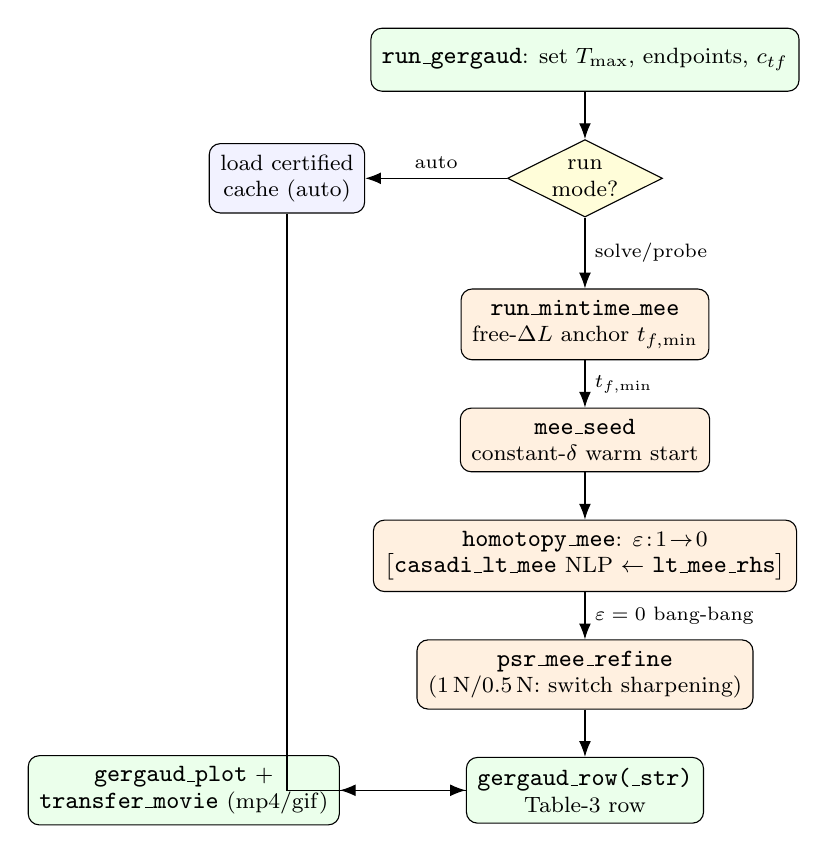
\begin{tikzpicture}[
  node distance=6mm and 10mm,
  box/.style={draw,rounded corners,align=center,font=\footnotesize,inner sep=4pt,minimum height=8mm,fill=blue!5},
  core/.style={box,fill=orange!12},
  io/.style={box,fill=green!8},
  dec/.style={draw,diamond,aspect=2,align=center,font=\footnotesize,inner sep=1pt,fill=yellow!15},
  a/.style={-{Latex[length=2mm]}}]

\node[io] (in) {\file{run\_gergaud}: set $\Tmax$, endpoints, $c_{tf}$};
\node[dec,below=of in] (mode) {run\\mode?};
\node[box,left=18mm of mode] (cache) {load certified\\cache (auto)};
\node[core,below=9mm of mode] (mt) {\file{run\_mintime\_mee}\\free-$\Delta L$ anchor $t_{f,\min}$};
\node[core,below=of mt] (seed) {\file{mee\_seed}\\ constant-$\delta$ warm start};
\node[core,below=of seed] (hom) {\file{homotopy\_mee}: $\varepsilon\!:\!1\!\to\!0$\\ $\big[$\file{casadi\_lt\_mee} NLP $\leftarrow$ \file{lt\_mee\_rhs}$\big]$};
\node[core,below=of hom] (psr) {\file{psr\_mee\_refine}\\ (1\,N/0.5\,N: switch sharpening)};
\node[io,below=of psr] (row) {\file{gergaud\_row(\_str)}\\ Table-3 row};
\node[io,left=16mm of row] (viz) {\file{gergaud\_plot} +\\ \file{transfer\_movie} (mp4/gif)};

\draw[a] (in) -- (mode);
\draw[a] (mode) -- node[above,font=\scriptsize]{auto} (cache);
\draw[a] (mode) -- node[right,font=\scriptsize]{solve/probe} (mt);
\draw[a] (mt) -- node[right,font=\scriptsize]{$t_{f,\min}$} (seed);
\draw[a] (seed) -- (hom);
\draw[a] (hom) -- node[right,font=\scriptsize]{$\varepsilon=0$ bang-bang} (psr);
\draw[a] (psr) -- (row);
\draw[a] (cache) |- (row);
\draw[a] (row) -- (viz);
\end{tikzpicture}
\caption{Generating one Table-3 row. Orange = live solve stages (skipped in
\texttt{auto} mode, which reuses a certified cache); green = input/output. The
NLP core \file{casadi\_lt\_mee} evaluates the MEE dynamics \file{lt\_mee\_rhs} at
every collocation node.}
\label{fig:flow}
\end{figure}

\begin{thebibliography}{9}
\bibitem{ghm2004} J.~Gergaud, T.~Haberkorn, and P.~Martinon,
``Low thrust minimum-fuel orbital transfer: a homotopic approach,''
\emph{Journal of Guidance, Control, and Dynamics}, 27(6), 2004.
\bibitem{be2002} R.~Bertrand and R.~\'Ep\'enoy,
``New smoothing techniques for solving bang-bang optimal control problems,''
\emph{Optimal Control Applications and Methods}, 23(4), 2002.
\bibitem{walker1985} M.~J.~H.~Walker, B.~Ireland, and J.~Owens,
``A set of modified equinoctial orbit elements,''
\emph{Celestial Mechanics}, 36(4), 1985.
\bibitem{betts2010} J.~T.~Betts, \emph{Practical Methods for Optimal Control and
Estimation Using Nonlinear Programming}, 2nd ed., SIAM, 2010.
\bibitem{kelly2017} M.~Kelly, ``An introduction to trajectory optimization: how
to do your own direct collocation,'' \emph{SIAM Review}, 59(4), 2017.
\end{thebibliography}

\end{document}
